% !TEX root = ../main.tex
\chapter{Basic Electronic Components \& Circuit Fundamentals}

\section{Taxonomy of Electronic Components}
Electronic components are the foundational physical building blocks of all electrical networks \cite{seymour_components, kalyanaraman_circuits}. Components are broadly classified by their energetic behavior into \textbf{passive} and \textbf{active} devices:

\begin{itemize}[leftmargin=1.5em]
    \item \textbf{Passive Components:} Devices that cannot deliver net power gain or inject external energy into a network. They dissipate, store, or release energy present in the circuit.
    \item \textbf{Active Components:} Devices that rely on an external power source to amplify electrical signals, control directional power flow, or provide electronic switching.
\end{itemize}

\section{Fundamental Passive Components}

\subsection{Resistors}
Resistors introduce precise electrical opposition to electric current, functioning to divide voltages, limit branch currents, and set active component bias operating points \cite{seymour_components}. Standard axial-lead resistors are fabricated using carbon film or metal film compositions, with values marked by standardized 4-band or 5-band color codes.

As current flows through a resistor, electrical energy is converted into thermal energy ($P = I^2 R = V \cdot I$). Consequently, resistors are categorized by their continuous physical power dissipation ratings:
\begin{itemize}[leftmargin=1.5em]
    \item \textbf{Standard Signal Resistors ($1/4\text{ W}$ and $1/2\text{ W}$):} Small cylindrical packages suitable for breadboard prototyping and low-power control lines.
    \item \textbf{Power Resistors ($1\text{ W}$ to $5\text{ W}+$):} Larger bodies, often encapsulated in white rectangular ceramic cement blocks, designed for power supplies and motor drivers.
\end{itemize}

\begin{figure}[htbp]
    \centering
    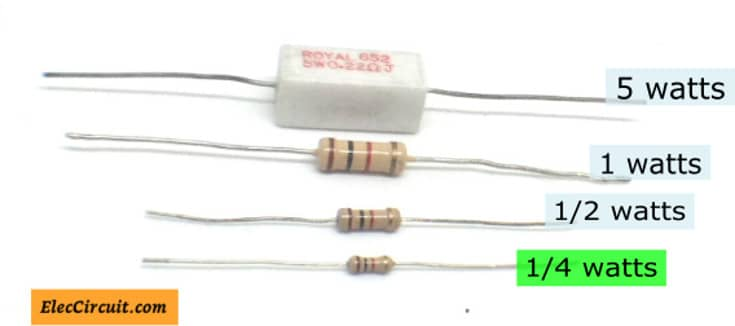
\includegraphics[width=0.72\textwidth]{figures/fig_resistors.jpg}
    \caption{Physical package comparison of resistors across various power ratings ($1/4\text{ W}$, $1/2\text{ W}$, $1\text{ W}$, and $5\text{ W}$ ceramic block) \cite{eleccircuit_components}.}
    \label{fig:resistors_power}
\end{figure}

\subsubsection{Schematic Symbols for Resistors}
In circuit schematics, resistors and their adjustable variants are depicted by standard symbols:

\begin{figure}[htbp]
    \centering
    \begin{tabular}{ccc}
        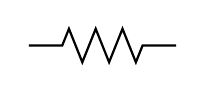
\begin{tikzpicture}[scale=0.85, baseline=-0.5ex]
            \draw[thick] (0,0) -- (0.5,0) -- (0.6,0.25) -- (0.8,-0.25) -- (1.0,0.25) -- (1.2,-0.25) -- (1.4,0.25) -- (1.6,-0.25) -- (1.7,0) -- (2.2,0);
        \end{tikzpicture}
        &
        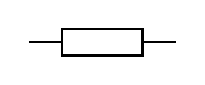
\begin{tikzpicture}[scale=0.85, baseline=-0.5ex]
            \draw[thick] (0,0) -- (0.5,0);
            \draw[thick, fill=white] (0.5,-0.2) rectangle (1.7,0.2);
            \draw[thick] (1.7,0) -- (2.2,0);
        \end{tikzpicture}
        &
        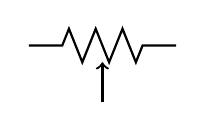
\begin{tikzpicture}[scale=0.85, baseline=-0.5ex]
            \draw[thick] (0,0) -- (0.5,0) -- (0.6,0.25) -- (0.8,-0.25) -- (1.0,0.25) -- (1.2,-0.25) -- (1.4,0.25) -- (1.6,-0.25) -- (1.7,0) -- (2.2,0);
            \draw[thick, ->] (1.1,-0.65) -- (1.1,-0.25);
            \draw[thick] (1.1,-0.65) -- (1.1,-0.85);
        \end{tikzpicture}
        \\
        \small \textbf{Fixed Resistor (US ANSI)} & \small \textbf{Fixed Resistor (IEC)} & \small \textbf{Potentiometer / Trimmer}
    \end{tabular}
    \caption{Standard schematic diagram symbols for fixed resistors and variable potentiometers.}
    \label{fig:resistor_symbols}
\end{figure}
\subsection{Capacitors}
Capacitors store electrical potential energy within an electrostatic field established between two conductive plates separated by an insulating dielectric medium. Capacitance is defined as:
\begin{equation}
    C = \frac{Q}{V}
\end{equation}
measured in Farads (F). In steady-state DC circuits, a charged capacitor behaves as an open circuit (blocking continuous DC current), while presenting low capacitive reactance ($X_C = \frac{1}{2\pi f C}$) to dynamic AC signals and transients.

\begin{figure}[htbp]
    \centering
    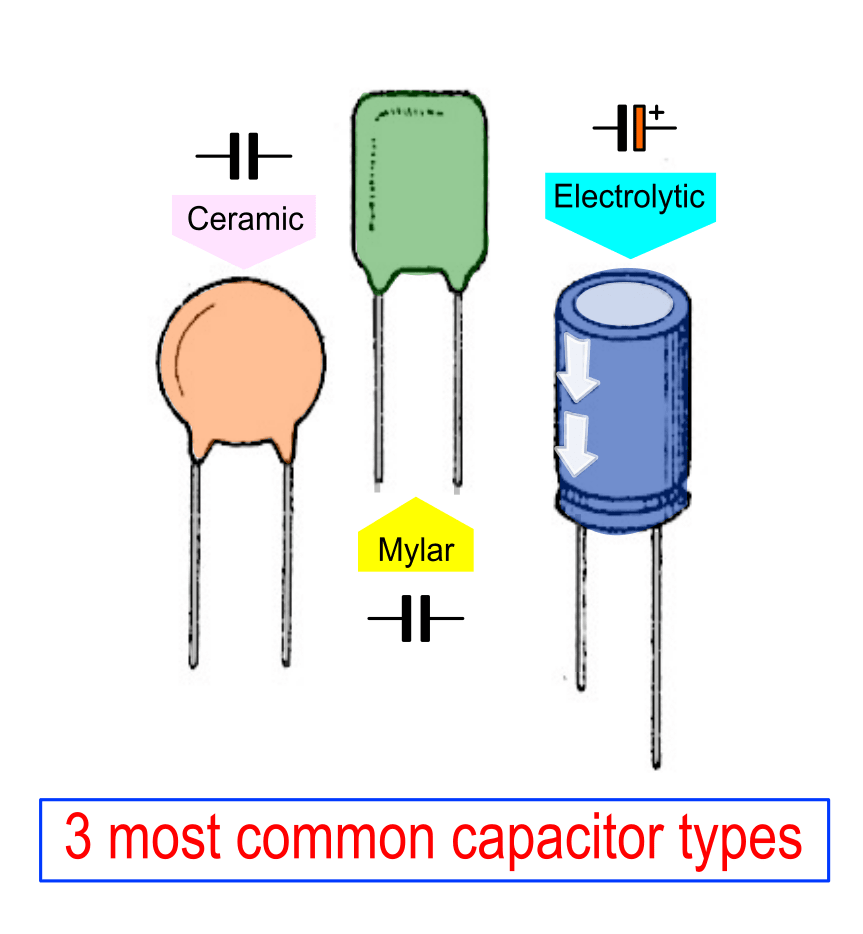
\includegraphics[width=0.72\textwidth]{figures/fig_capacitors.png}
    \caption{Three common capacitor types used in laboratory prototypes: Electrolytic, Ceramic, and Mylar \cite{eleccircuit_components}.}
    \label{fig:capacitors_types}
\end{figure}

\subsubsection{Capacitor Types, Polarity \& Marking Schemes}
\begin{itemize}[leftmargin=1.5em]
    \item \textbf{Electrolytic Capacitors (Polarized):} Feature high capacitance density ($0.1\ \mu\text{F}$ to $>10{,}000\ \mu\text{F}$). \textbf{Polarity is mandatory:} the negative lead is shorter and marked with a prominent white/gray stripe with minus signs ($-$). Connecting an electrolytic capacitor in reverse polarity can cause electrolyte boiling, gas venting, or catastrophic failure.
    \item \textbf{Ceramic and Mylar Capacitors (Non-Polarized):} Smaller capacitance values (picofarads to tenths of a microfarad) without polarity constraints.
    \item \textbf{3-Digit EIA Marking Code:} Non-polarized capacitors use a 3-digit numerical code in picofarads (pF):
    \begin{itemize}[leftmargin=1.2em]
        \item The first two digits represent the significant base value.
        \item The third digit represents the multiplier ($10^n$).
        \item \textit{Example:} A capacitor labeled \textbf{104} translates to $10 \times 10^4\text{ pF} = 100{,}000\text{ pF} = 0.1\ \mu\text{F}$.
    \end{itemize}
\end{itemize}

\subsubsection{Schematic Symbols for Capacitors}
\begin{figure}[htbp]
    \centering
    \begin{tabular}{ccc}
        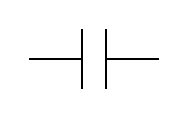
\begin{tikzpicture}[scale=0.85, baseline=-0.5ex]
            \draw[thick] (0,0) -- (0.8,0);
            \draw[thick] (0.8,0.45) -- (0.8,-0.45);
            \draw[thick] (1.15,0.45) -- (1.15,-0.45);
            \draw[thick] (1.15,0) -- (1.95,0);
        \end{tikzpicture}
        &
        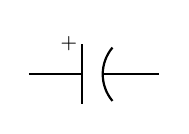
\begin{tikzpicture}[scale=0.85, baseline=-0.5ex]
            \draw[thick] (0,0) -- (0.8,0);
            \draw[thick] (0.8,0.45) -- (0.8,-0.45);
            \draw[thick] (1.25,0.4) arc (140:220:0.62);
            \draw[thick] (1.12,0) -- (1.95,0);
            \node[above, font=\scriptsize\bfseries] at (0.6,0.2) {$+$};
        \end{tikzpicture}
        &
        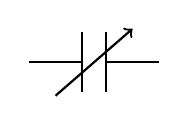
\begin{tikzpicture}[scale=0.85, baseline=-0.5ex]
            \draw[thick] (0,0) -- (0.8,0);
            \draw[thick] (0.8,0.45) -- (0.8,-0.45);
            \draw[thick] (1.15,0.45) -- (1.15,-0.45);
            \draw[thick] (1.15,0) -- (1.95,0);
            \draw[thick, ->] (0.4,-0.5) -- (1.55,0.5);
        \end{tikzpicture}
        \\
        \small \textbf{Non-Polarized Capacitor} & \small \textbf{Polarized (Electrolytic)} & \small \textbf{Variable Capacitor}
    \end{tabular}
    \caption{Standard schematic diagram symbols for non-polarized, polarized electrolytic, and variable capacitors.}
    \label{fig:capacitor_symbols}
\end{figure}
\subsection{Inductors \& Electromagnetic Energy Storage}
Inductors consist of insulated conductive wire wound into a helical coil around a magnetic core (ferrite, iron, or air). Inductors store energy within a concentrated magnetic field established by flowing current. The induced counter-electromotive force opposes instantaneous current fluctuations according to Faraday's and Lenz's laws:
\begin{equation}
    V = L \cdot \frac{di}{dt}
\end{equation}
where $L$ is inductance measured in Henries (H). Inductors resist abrupt changes in current, making them essential for switching regulator LC filters, choke suppression, and RF tuning networks.

\subsubsection{Schematic Symbols for Inductors}
\begin{figure}[htbp]
    \centering
    \begin{tabular}{ccc}
        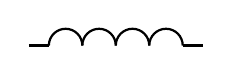
\begin{tikzpicture}[scale=0.85, baseline=-0.5ex]
            \draw[thick] (0,0) -- (0.3,0);
            \draw[thick] (0.3,0) arc (180:0:0.25);
            \draw[thick] (0.8,0) arc (180:0:0.25);
            \draw[thick] (1.3,0) arc (180:0:0.25);
            \draw[thick] (1.8,0) arc (180:0:0.25);
            \draw[thick] (2.3,0) -- (2.6,0);
        \end{tikzpicture}
        &
        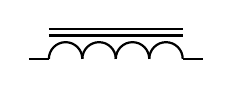
\begin{tikzpicture}[scale=0.85, baseline=-0.5ex]
            \draw[thick] (0,0) -- (0.3,0);
            \draw[thick] (0.3,0) arc (180:0:0.25);
            \draw[thick] (0.8,0) arc (180:0:0.25);
            \draw[thick] (1.3,0) arc (180:0:0.25);
            \draw[thick] (1.8,0) arc (180:0:0.25);
            \draw[thick] (2.3,0) -- (2.6,0);
            \draw[thick] (0.3,0.35) -- (2.3,0.35);
            \draw[thick] (0.3,0.45) -- (2.3,0.45);
        \end{tikzpicture}
        &
        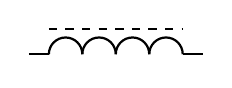
\begin{tikzpicture}[scale=0.85, baseline=-0.5ex]
            \draw[thick] (0,0) -- (0.3,0);
            \draw[thick] (0.3,0) arc (180:0:0.25);
            \draw[thick] (0.8,0) arc (180:0:0.25);
            \draw[thick] (1.3,0) arc (180:0:0.25);
            \draw[thick] (1.8,0) arc (180:0:0.25);
            \draw[thick] (2.3,0) -- (2.6,0);
            \draw[thick, dashed] (0.3,0.38) -- (2.3,0.38);
        \end{tikzpicture}
        \\
        \small \textbf{Air-Core Inductor} & \small \textbf{Iron-Core Inductor} & \small \textbf{Ferrite-Core Inductor}
    \end{tabular}
    \caption{Standard schematic diagram symbols for inductors with air, iron, and ferrite cores.}
    \label{fig:inductor_symbols}
\end{figure}
\section{Electrical Impedance and AC Circuit Dynamics}
While direct-current (DC) analysis evaluates circuits strictly through ohmic resistance ($R$), alternating-current (AC) signals introduce dynamic electromagnetic and electrostatic behaviors. The generalized opposition that an electrical network presents to the flow of sinusoidal alternating current is known as \textbf{electrical impedance} ($Z$).

Impedance is expressed mathematically as a complex number in rectangular and polar forms:
\begin{equation}
    Z = R + jX = |Z|\angle\theta
\end{equation}
where $j = \sqrt{-1}$ is the imaginary unit, and:
\begin{itemize}[leftmargin=1.5em]
    \item \textbf{Resistance ($R$):} The real part of impedance, measured in ohms ($\Omega$). It represents the irreversible dissipation of electrical energy into thermal heat ($P = I_{\text{rms}}^2 R$), occurring independently of signal frequency in ideal components.
    \item \textbf{Reactance ($X$):} The imaginary part of impedance, measured in ohms ($\Omega$). It represents the reversible storage and release of energy within electric fields (capacitive reactance, $X_C$) or magnetic fields (inductive reactance, $X_L$). Unlike resistance, reactance is strictly frequency-dependent.
    \item \textbf{Impedance Magnitude ($|Z|$):} The ratio of peak voltage to peak current:
    \begin{equation}
        |Z| = \sqrt{R^2 + X^2}
    \end{equation}
    \item \textbf{Phase Angle ($\theta$):} The temporal phase shift between voltage and current waveforms:
    \begin{equation}
        \theta = \arctan\left(\frac{X}{R}\right)
    \end{equation}
\end{itemize}

\subsection{Capacitive Reactance (\texorpdfstring{$X_C$}{X\_C})}
A capacitor opposes changes in voltage by accumulating electrostatic charge on its conductive plates. When subjected to a sinusoidal voltage with angular frequency $\omega = 2\pi f$, its complex impedance is given by:
\begin{equation}
    Z_C = \frac{1}{j\omega C} = -j\frac{1}{\omega C} = -j X_C
\end{equation}
where capacitive reactance is:
\begin{equation}
    X_C = \frac{1}{\omega C} = \frac{1}{2\pi f C}
\end{equation}
At zero frequency (DC, $f = 0$), $X_C \to \infty$, causing the capacitor to behave as an open circuit (blocking DC bias). As frequency increases, $X_C \to 0$, causing the capacitor to behave as an AC short circuit. This inverse frequency relationship forms the foundation of power supply decoupling, where capacitors shunt high-frequency transient noise to ground while preserving DC rails. In a pure capacitor, current leads voltage by $90^\circ$ ($\pi/2\text{ rad}$).

\subsection{Inductive Reactance (\texorpdfstring{$X_L$}{X\_L})}
An inductor opposes changes in current through the self-induction of counter-electromotive force (Lenz's Law). When driven by an alternating current, its complex impedance is:
\begin{equation}
    Z_L = j\omega L = +j X_L
\end{equation}
where inductive reactance is:
\begin{equation}
    X_L = \omega L = 2\pi f L
\end{equation}
At zero frequency (DC, $f = 0$), $X_L = 0\,\Omega$, allowing direct current to pass through with zero theoretical opposition. As frequency increases, $X_L$ scales linearly, presenting massive impedance to high-frequency AC signals. This direct frequency scaling allows inductors to function as electromagnetic interference (EMI) chokes and low-pass filtering elements. In a pure inductor, voltage leads current by $90^\circ$ ($\pi/2\text{ rad}$).

\subsection{Practical Engineering Applications of Impedance}
\begin{itemize}[leftmargin=1.5em]
    \item \textbf{Passive Frequency Filters:} Combining resistors with reactive elements produces frequency-selective networks, including RC/RL first-order low-pass filters (cut-off frequency $f_c = \frac{1}{2\pi RC}$) and high-pass filters used extensively in audio processing, sensor conditioning, and analog-to-digital converter (ADC) anti-aliasing.
    \item \textbf{Impedance Matching \& Signal Integrity:} In high-speed digital communications and RF systems, circuit traces behave as transmission lines. When the load impedance does not match the source and line characteristic impedance (typically $50\,\Omega$ in RF and $100\,\Omega$ differential in USB/Ethernet), signal reflections occur, generating ringing, false logic triggers, and severe data degradation.
\end{itemize}

\section{Active Semiconductor Devices}

\subsection{Diodes}
A semiconductor diode consists of a $p$-$n$ junction that acts as an electrical one-way valve for current flow. When forward-biased ($V > V_F$), current flows freely from \textbf{Anode ($A$)} to \textbf{Cathode ($K$)}. Under reverse bias, current flow is blocked.

\begin{figure}[htbp]
    \centering
    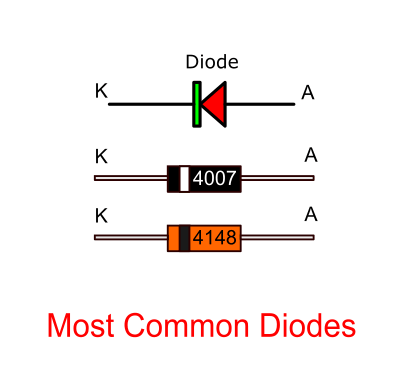
\includegraphics[width=0.68\textwidth]{figures/fig_diodes.png}
    \caption{Common semiconductor diodes (1N4007 power rectifier, 1N4148 high-speed signal) with physical cathode identification bands and corresponding schematic symbol \cite{eleccircuit_components}.}
    \label{fig:diodes_common}
\end{figure}

\subsubsection{Cathode Identification \& Types of Diodes}
\begin{itemize}[leftmargin=1.5em]
    \item \textbf{Cathode Marking Band:} On physical diode cylinders (such as the black epoxy 1N4007 or glass DO-35 1N4148), a painted silver or black band denotes the \textbf{Cathode ($K$)} terminal.
    \item \textbf{Zener Diodes:} Designed to operate in reverse breakdown at a stable, specified Zener voltage ($V_Z$), providing constant voltage regulation.
\end{itemize}

\begin{figure}[htbp]
    \centering
    \begin{tabular}{ccc}
        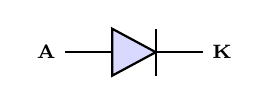
\begin{tikzpicture}[scale=0.85, baseline=-0.5ex]
            \draw[thick] (0,0) -- (0.7,0);
            \draw[thick, fill=blue!15] (0.7,0.35) -- (0.7,-0.35) -- (1.35,0) -- cycle;
            \draw[thick] (1.35,0.35) -- (1.35,-0.35);
            \draw[thick] (1.35,0) -- (2.05,0);
            \node[left, font=\scriptsize\bfseries] at (0,0) {A};
            \node[right, font=\scriptsize\bfseries] at (2.05,0) {K};
        \end{tikzpicture}
        &
        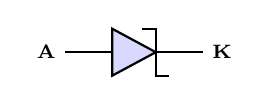
\begin{tikzpicture}[scale=0.85, baseline=-0.5ex]
            \draw[thick] (0,0) -- (0.7,0);
            \draw[thick, fill=blue!15] (0.7,0.35) -- (0.7,-0.35) -- (1.35,0) -- cycle;
            \draw[thick] (1.15,0.35) -- (1.35,0.35) -- (1.35,-0.35) -- (1.55,-0.35);
            \draw[thick] (1.35,0) -- (2.05,0);
            \node[left, font=\scriptsize\bfseries] at (0,0) {A};
            \node[right, font=\scriptsize\bfseries] at (2.05,0) {K};
        \end{tikzpicture}
        &
        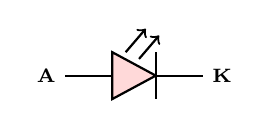
\begin{tikzpicture}[scale=0.85, baseline=-0.5ex]
            \draw[thick] (0,0) -- (0.7,0);
            \draw[thick, fill=red!15] (0.7,0.35) -- (0.7,-0.35) -- (1.35,0) -- cycle;
            \draw[thick] (1.35,0.35) -- (1.35,-0.35);
            \draw[thick] (1.35,0) -- (2.05,0);
            \draw[thick, ->] (0.9,0.35) -- (1.2,0.7);
            \draw[thick, ->] (1.1,0.25) -- (1.4,0.6);
            \node[left, font=\scriptsize\bfseries] at (0,0) {A};
            \node[right, font=\scriptsize\bfseries] at (2.05,0) {K};
        \end{tikzpicture}
        \\
        \small \textbf{Standard Diode} & \small \textbf{Zener Diode} & \small \textbf{Light Emitting Diode (LED)}
    \end{tabular}
    \caption{Schematic symbols for standard $p$-$n$ junction diodes, Zener voltage regulation diodes, and LEDs with emission rays.}
    \label{fig:diode_symbols}
\end{figure}
\subsection{Light Emitting Diodes (LEDs)}
Light Emitting Diodes (LEDs) are specialized $p$-$n$ junction diodes that emit light through electroluminescence when forward-biased. Because an unbuffered LED behaves as a near short-circuit once forward voltage threshold is exceeded, a series current-limiting resistor is mandatory.

\begin{figure}[htbp]
    \centering
    \begin{minipage}{0.48\textwidth}
        \centering
        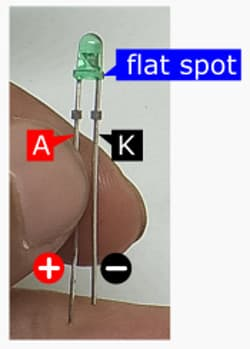
\includegraphics[width=\textwidth]{figures/fig_led_pinout.jpg}
        \caption{Physical pinout features of a standard LED: longer lead is Anode ($+$), shorter lead and flat rim spot indicate Cathode ($-$) \cite{eleccircuit_leds}.}
        \label{fig:led_pinout}
    \end{minipage}\hfill
    \begin{minipage}{0.48\textwidth}
        \centering
        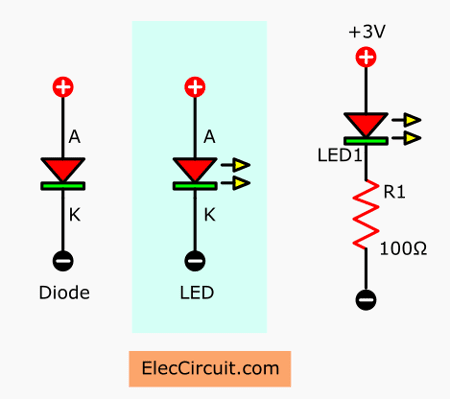
\includegraphics[width=\textwidth]{figures/fig_led_symbol.png}
        \caption{Schematic symbol of an LED showing current direction ($A \rightarrow K$) and outward radiation arrows \cite{eleccircuit_leds}.}
        \label{fig:led_symbol}
    \end{minipage}
\end{figure}

\subsubsection{LED Forward Voltages \& Polarity Rules}
\begin{itemize}[leftmargin=1.5em]
    \item \textbf{Polarity Verification:}
    \begin{itemize}[leftmargin=1.2em]
        \item \textbf{Lead Length:} The longer lead is the \textbf{Anode ($+$)}, and the shorter lead is the \textbf{Cathode ($-$/GND)}.
        \item \textbf{Flat Spot on Lens Rim:} When leads are trimmed, look for the flat edge molded onto the plastic lens perimeter; this always designates the \textbf{Cathode ($-$/K)}.
    \end{itemize}
    \item \textbf{Typical Forward Voltages ($V_F$):} Red ($\approx 1.7\text{ V}$), Yellow/Green ($\approx 2.1\text{--}2.3\text{ V}$), Blue/White ($\approx 3.3\text{--}3.6\text{ V}$).
\end{itemize}

\subsection{Transistors: BJT and MOSFET Architecture}
Transistors function as electronically controlled switches and current/voltage amplifiers:

\begin{figure}[htbp]
    \centering
    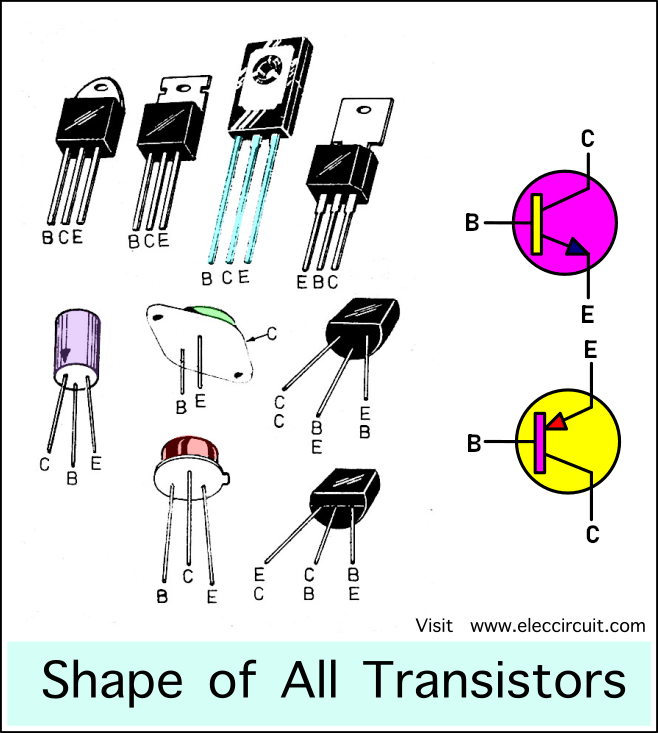
\includegraphics[width=0.75\textwidth]{figures/fig_transistor_shapes.png}
    \caption{Common physical transistor packages (TO-92, TO-220, TO-126) with terminal pinouts (B-C-E), and standard BJT schematic symbols (NPN vs. PNP) \cite{eleccircuit_components}.}
    \label{fig:transistor_shapes}
\end{figure}

\subsubsection{Bipolar Junction Transistors (BJTs)}
BJTs are 3-terminal, current-controlled devices comprising Base ($B$), Collector ($C$), and Emitter ($E$):
\begin{equation}
    I_C = \beta \cdot I_B
\end{equation}
where $\beta$ ($h_{FE}$) is the common-emitter forward current gain.
\begin{figure}[htbp]
    \centering
    \begin{tabular}{cc}
        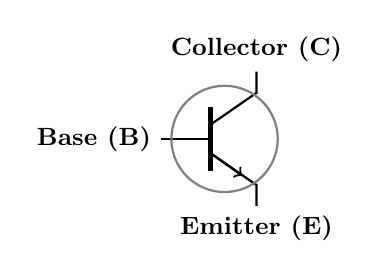
\begin{tikzpicture}[scale=0.9, baseline=-0.5ex]
            \draw[thick] (0,0) -- (0.7,0);
            \draw[ultra thick] (0.7,-0.45) -- (0.7,0.45);
            \draw[thick] (0.7,0.2) -- (1.35,0.65) -- (1.35,0.95);
            \draw[thick] (0.7,-0.2) -- (1.35,-0.65) -- (1.35,-0.95);
            \draw[thick, ->] (0.7,-0.2) -- (1.15,-0.52);
            \draw[thick, gray] (0.9,0) circle (0.75);
            \node[left, font=\small\bfseries] at (0,0) {Base (B)};
            \node[above, font=\small\bfseries] at (1.35,0.95) {Collector (C)};
            \node[below, font=\small\bfseries] at (1.35,-0.95) {Emitter (E)};
        \end{tikzpicture}
        &
        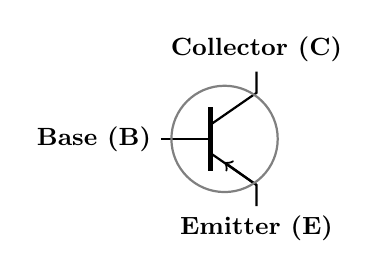
\begin{tikzpicture}[scale=0.9, baseline=-0.5ex]
            \draw[thick] (0,0) -- (0.7,0);
            \draw[ultra thick] (0.7,-0.45) -- (0.7,0.45);
            \draw[thick] (0.7,0.2) -- (1.35,0.65) -- (1.35,0.95);
            \draw[thick] (0.7,-0.2) -- (1.35,-0.65) -- (1.35,-0.95);
            \draw[thick, <-] (0.9,-0.33) -- (1.35,-0.65);
            \draw[thick, gray] (0.9,0) circle (0.75);
            \node[left, font=\small\bfseries] at (0,0) {Base (B)};
            \node[above, font=\small\bfseries] at (1.35,0.95) {Collector (C)};
            \node[below, font=\small\bfseries] at (1.35,-0.95) {Emitter (E)};
        \end{tikzpicture}
        \\
        \small \textbf{NPN BJT (Arrow Outward)} & \small \textbf{PNP BJT (Arrow Inward)}
    \end{tabular}
    \caption{Schematic symbols for NPN and PNP bipolar junction transistors, illustrating terminal designations and emitter current direction arrows.}
    \label{fig:bjt_symbols}
\end{figure}

\begin{itemize}[leftmargin=1.5em]
    \item \textbf{NPN Transistor:} Operates with positive collector voltage. The schematic symbol features an emitter arrow pointing \textbf{outward} (mnemonic: ``\textbf{N}ot \textbf{P}ointing i\textbf{N}'').
    \item \textbf{PNP Transistor:} Operates with negative collector bias. The schematic symbol features an emitter arrow pointing \textbf{inward} (mnemonic: ``\textbf{P}ointing i\textbf{N} \textbf{P}roudly'').
    \item \textbf{Terminal Pinouts:} Always verify package pinout specifications (e.g., E-B-C or B-C-E) because identical-looking TO-92 packages vary across transistor models.
\end{itemize}
\subsubsection{Field-Effect Transistors (MOSFETs)}
MOSFETs are voltage-controlled devices with near-infinite input impedance at DC. The voltage between Gate ($G$) and Source ($S$) creates an electric field modulating conductivity through the Drain ($D$) to Source channel.

\subsection{Integrated Circuits (ICs)}
Integrated Circuits (ICs) consolidate hundreds to millions of interconnected components onto a monolithic silicon die.

\begin{figure}[htbp]
    \centering
    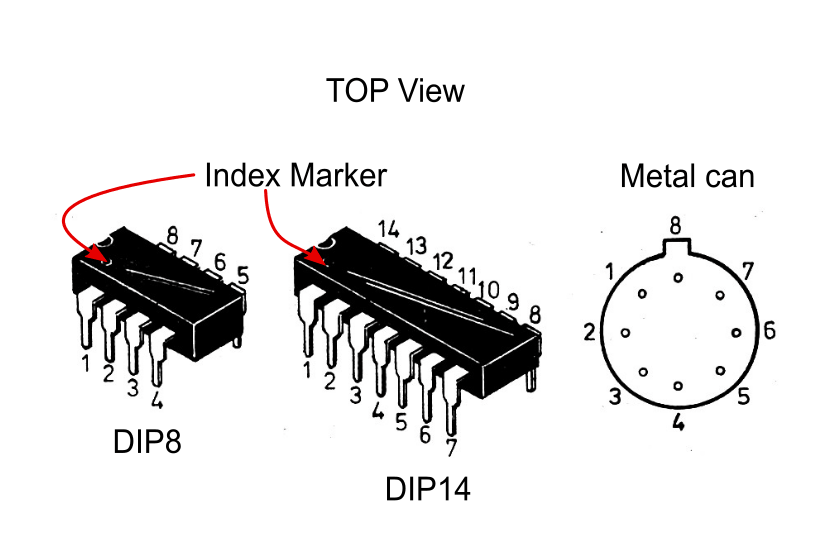
\includegraphics[width=0.75\textwidth]{figures/fig_ic_packages.png}
    \caption{Most common through-hole IC packages (DIP8, DIP14, and circular metal can) with index markers for pin numbering \cite{eleccircuit_components}.}
    \label{fig:ic_packages}
\end{figure}

\subsubsection{Pin Numbering Convention}
Through-hole Dual In-Line Packages (DIP8, DIP14, DIP16) follow a universal orientation standard:
\begin{enumerate}[leftmargin=1.5em]
    \item Locate the \textbf{index marker} (a semicircular notch or impressed dot) on the top face of the chip.
    \item Orient the notch facing to the left (or upward).
    \item Pin 1 is immediately to the left of the notch (or directly adjacent to the dot).
    \item Numbering increments \textbf{counter-clockwise} around the perimeter of the chip package, finishing at the top-left pin directly opposite Pin 1.
\end{enumerate}
\section{Series vs. Parallel Circuit Topologies}

\subsection{Series Circuits}
In a series topology, components are chained end-to-end along a single continuous path:
\begin{itemize}[leftmargin=1.5em]
    \item The current is identical through every component: $I_{total} = I_1 = I_2 = \dots = I_n$.
    \item Equivalent resistance is additive: $R_{eq} = \sum_{k=1}^n R_k$.
    \item Total voltage equals the sum of individual voltage drops (Kirchhoff's Voltage Law).
\end{itemize}

\subsection{Parallel Circuits}
In a parallel topology, components connect across two shared electrical nodes:
\begin{itemize}[leftmargin=1.5em]
    \item The voltage across every parallel branch is identical: $V_{total} = V_1 = V_2 = \dots = V_n$.
    \item Equivalent resistance is given by:
    \begin{equation}
        \frac{1}{R_{eq}} = \sum_{k=1}^n \frac{1}{R_k}
    \end{equation}
    \item Total current is the sum of branch currents (Kirchhoff's Current Law).
\end{itemize}
